\documentclass[a4paper, 12pt]{article}

\usepackage{babel}
\usepackage{enumitem}
\usepackage{times}
\usepackage{graphicx}
\usepackage{geometry}
	\geometry{left = 4cm, top = 4cm, right = 3cm, bottom = 3cm}
\usepackage{float}
\usepackage{setspace}
	\setstretch{1.5}
\usepackage{listings}
\usepackage{hyperref}


\begin{document}
\title{\huge\textbf{RESUME PRAKTEK APLIKASI APEX ORACLE}}
\date{}

\maketitle


\begin{figure}[!ht]
\begin{center}

\includegraphics[width = 5cm, height = 4.5cm]{gambar/logo.png}
\end{center}
\end{figure}

\begin{center}
\vspace{1cm}
Disusun oleh :\\
Syabriena Putri Veriane\\
D4 TI 2B\\
1.18.4.094\\
\vspace{1cm}
\textbf{PROGRAM DIPLOMA IV POLITEKNIK POS INDONESIA} \linebreak
\textbf{POLITEKNIK POS INDONESIA} \linebreak
\textbf{BANDUNG}\linebreak
\textbf{2019}

\end{center}

\thispagestyle{empty}

\clearpage
\setcounter{page}{1}

\section{Tutorial}

\begin{enumerate}

\item Login Oracle Apex\\
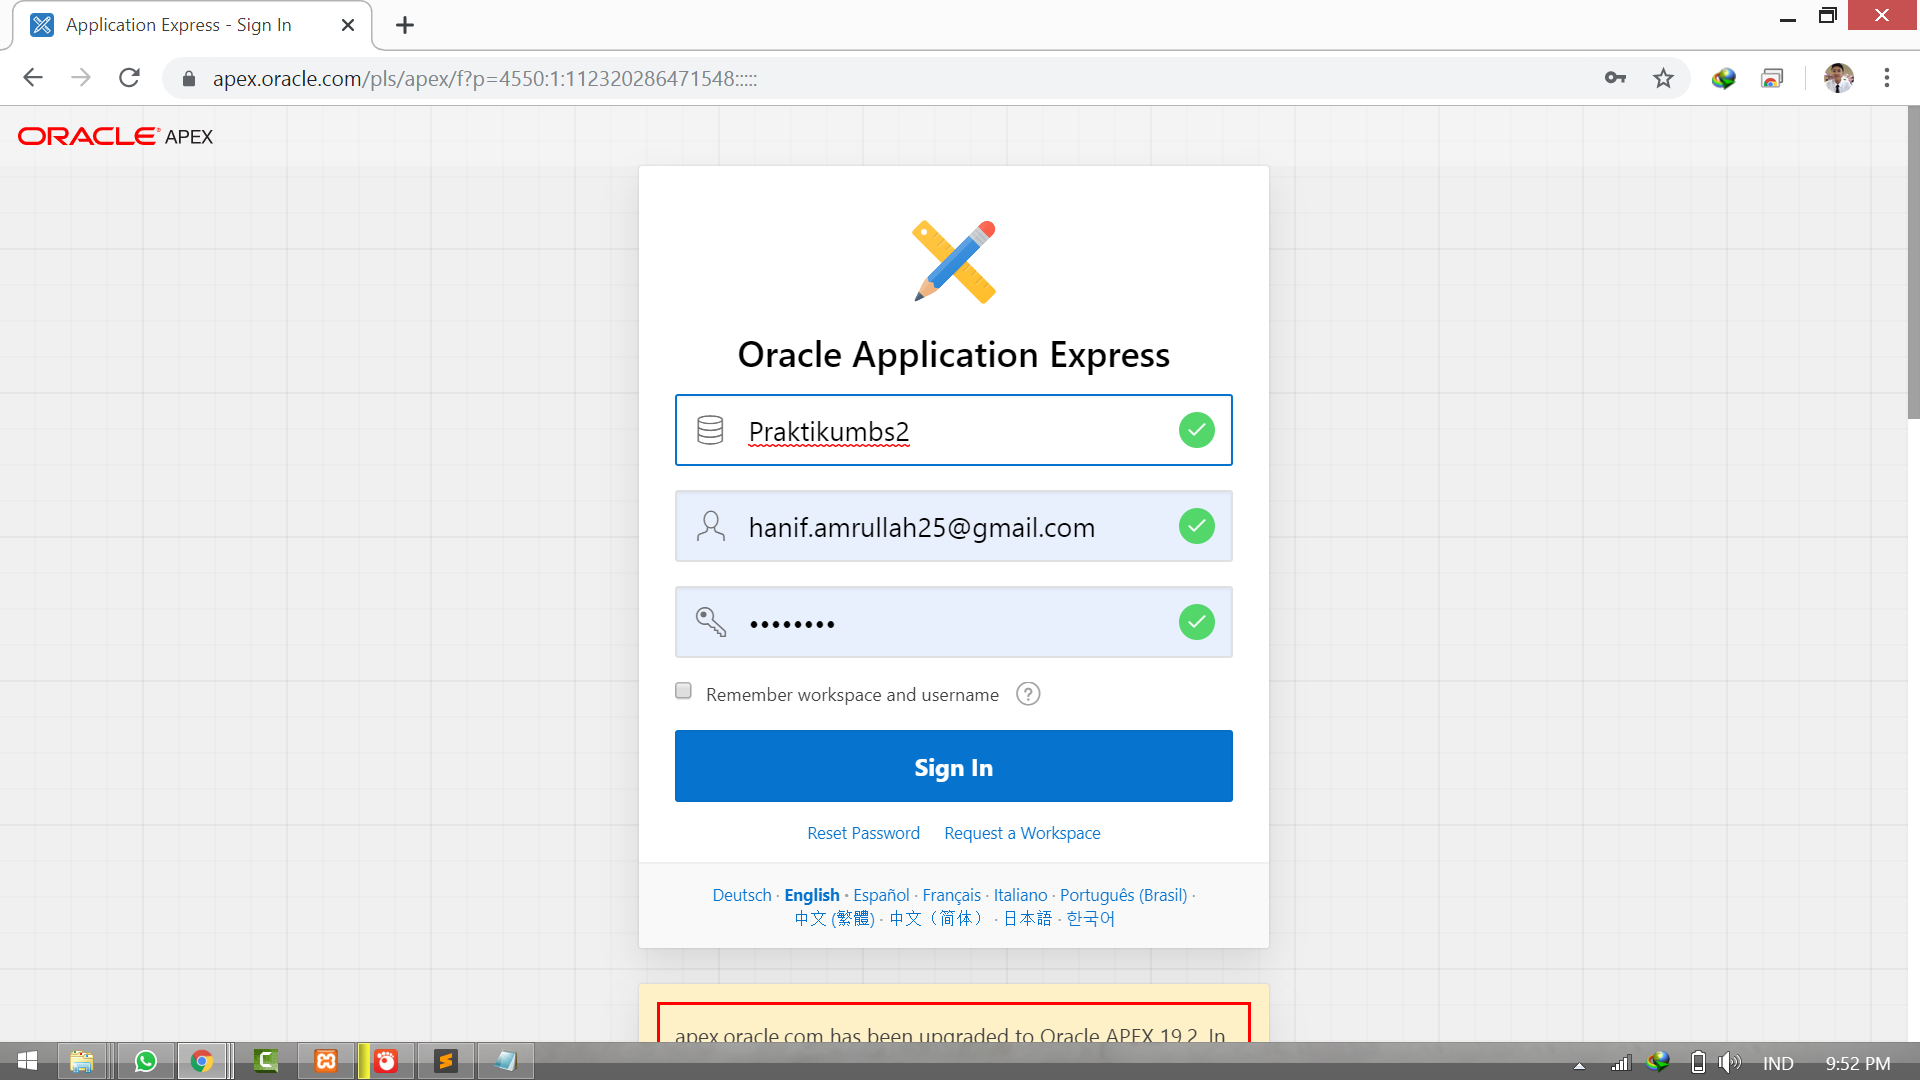
\includegraphics[scale = 0.3]{gambar/1.png}

\item Klik App Builder kemudian Create an Application dan pilih From a File. Pastikan file yang akan ditambahkan ada dan sudah berupa tabel tabel yang dinormalisasi dengan format csv. \\
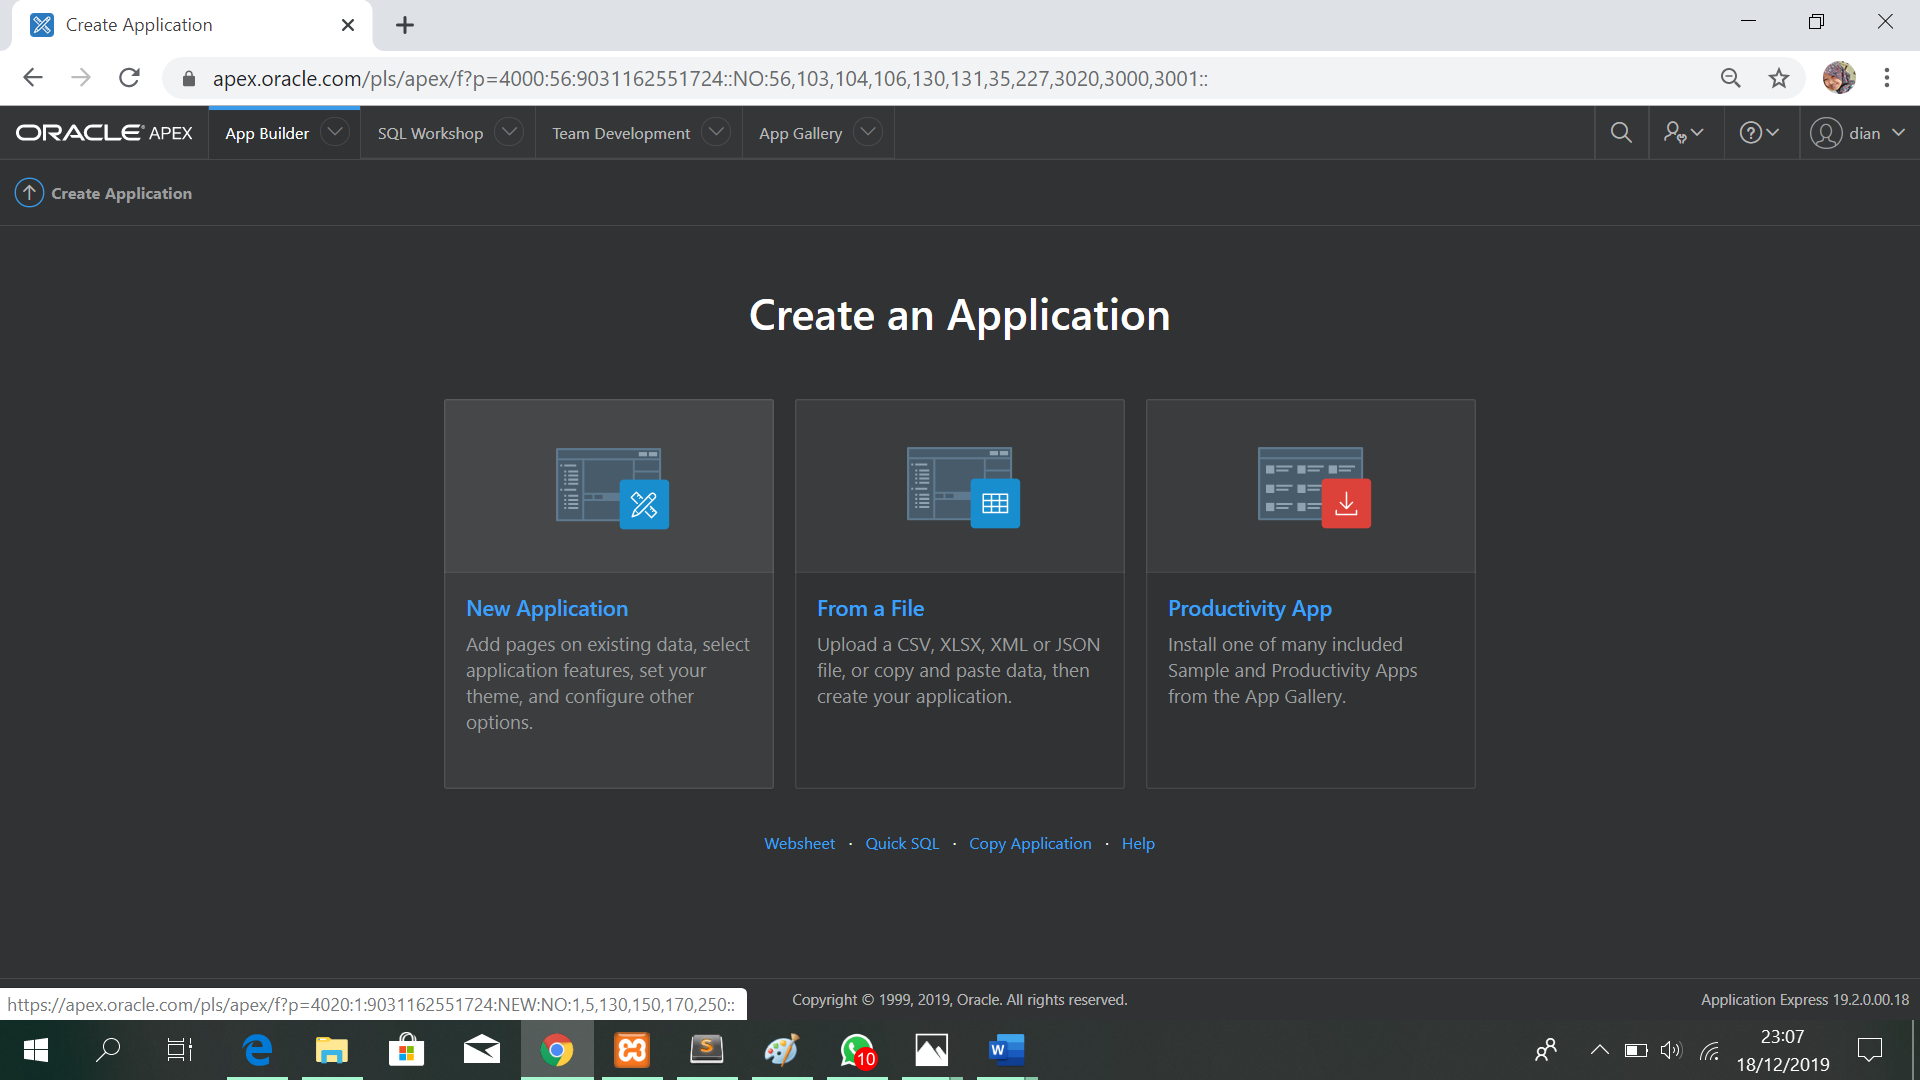
\includegraphics[scale = 0.3]{gambar/2.png}

\item Masukan Table Name dan Error Table Name\\
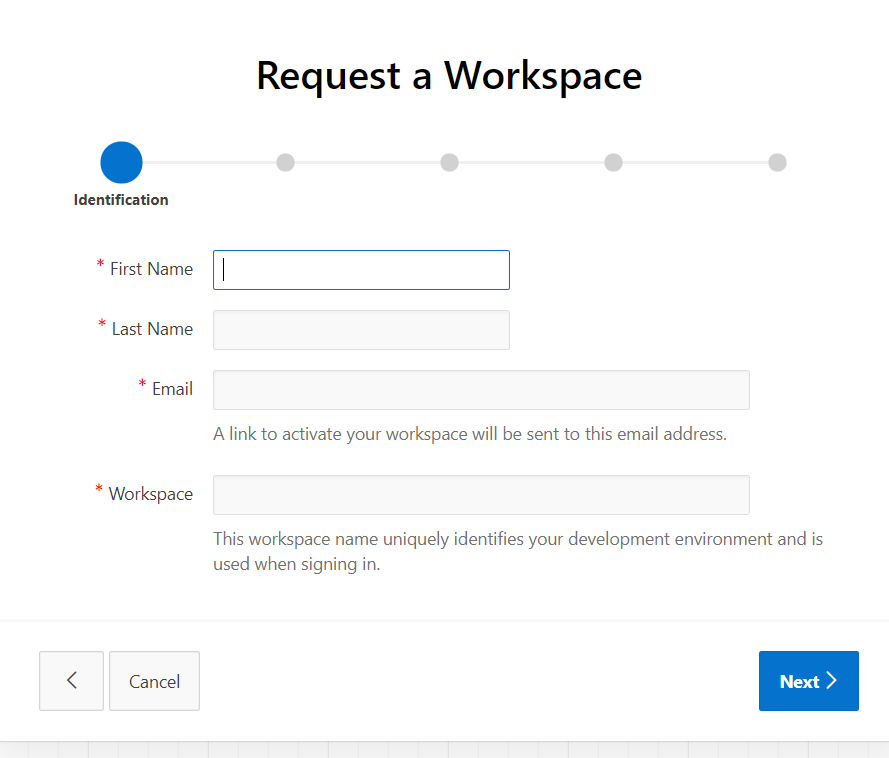
\includegraphics[scale = 0.3]{gambar/3.png}

\item Klik configure untuk mengkonfigurasi. Kemudian save change.\\
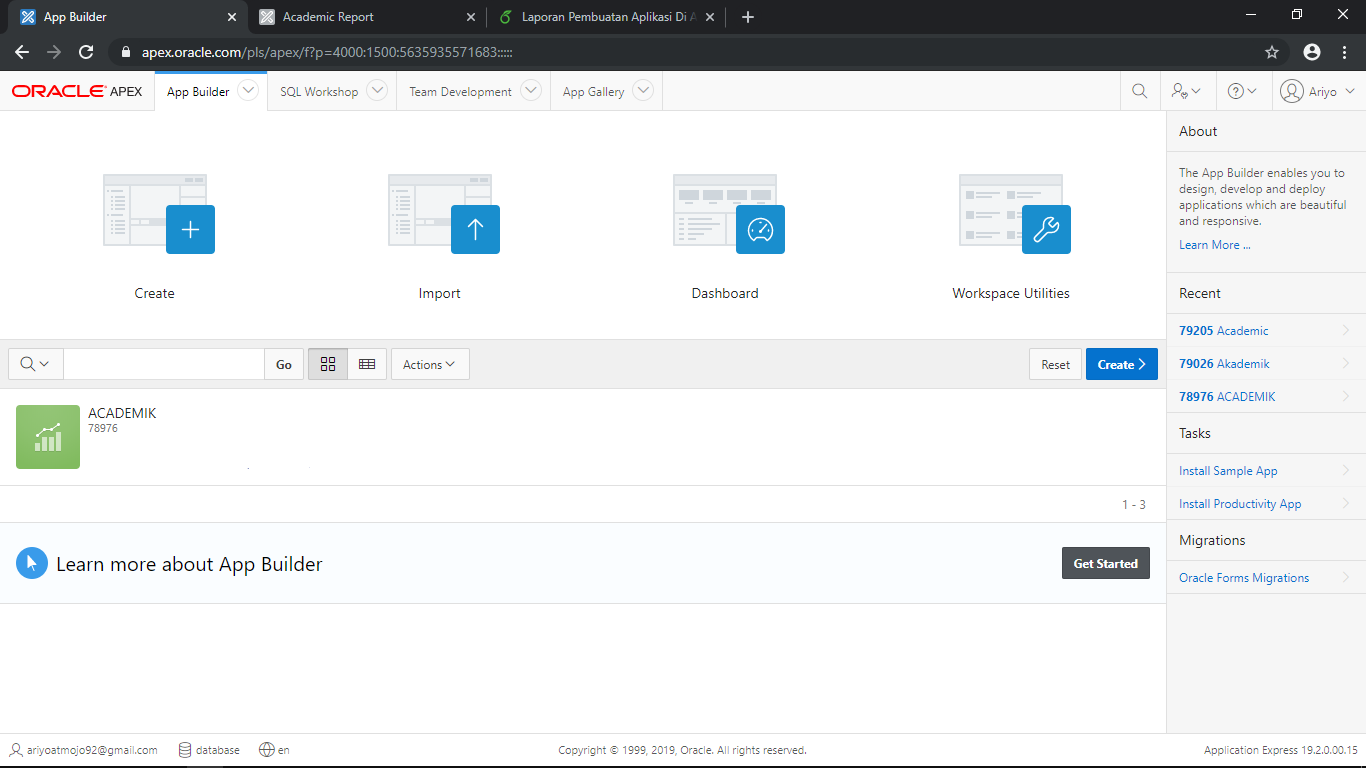
\includegraphics[scale = 0.3]{gambar/4.png}

\item Lakukan cara yang sama pada semua file yang akan di upload. Kemudian klik load data.\\
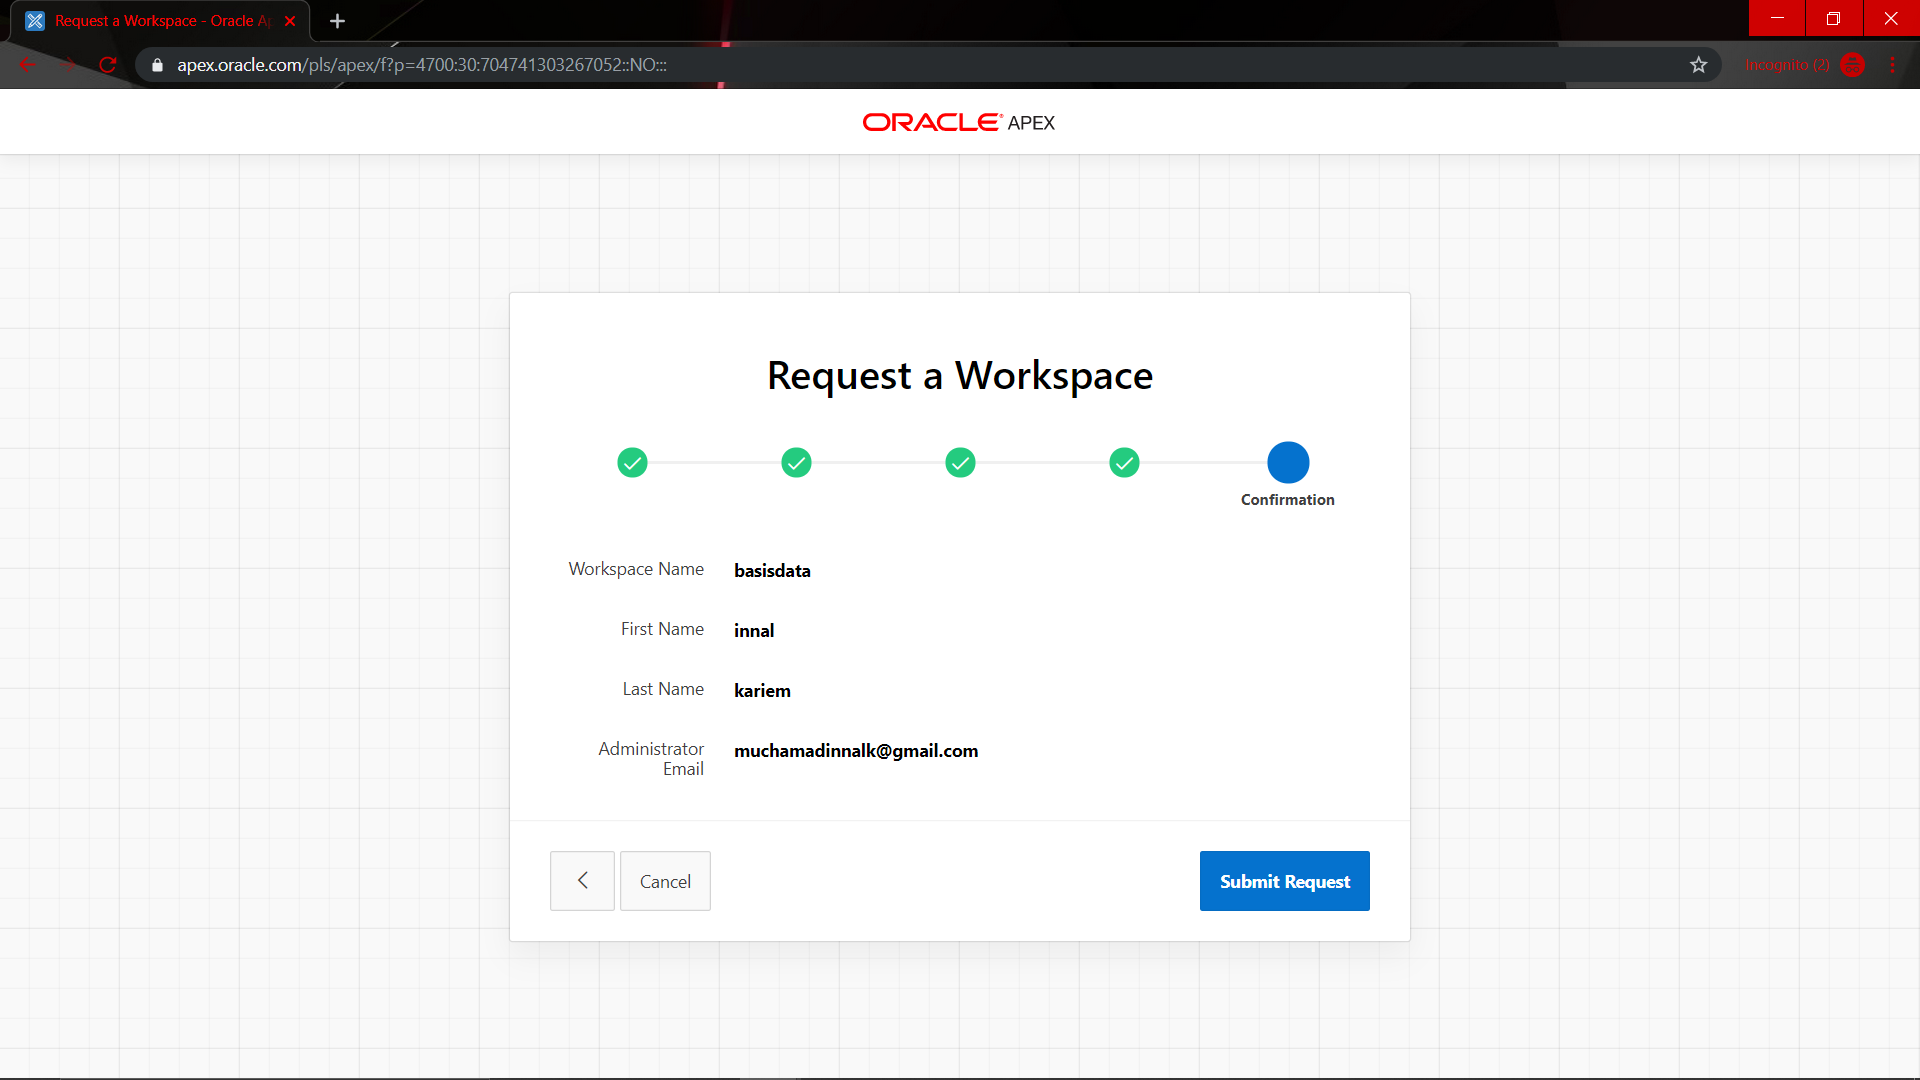
\includegraphics[scale = 0.3]{gambar/5.png}

\item Akan muncul windows seperti ini, kemudian tutup \\
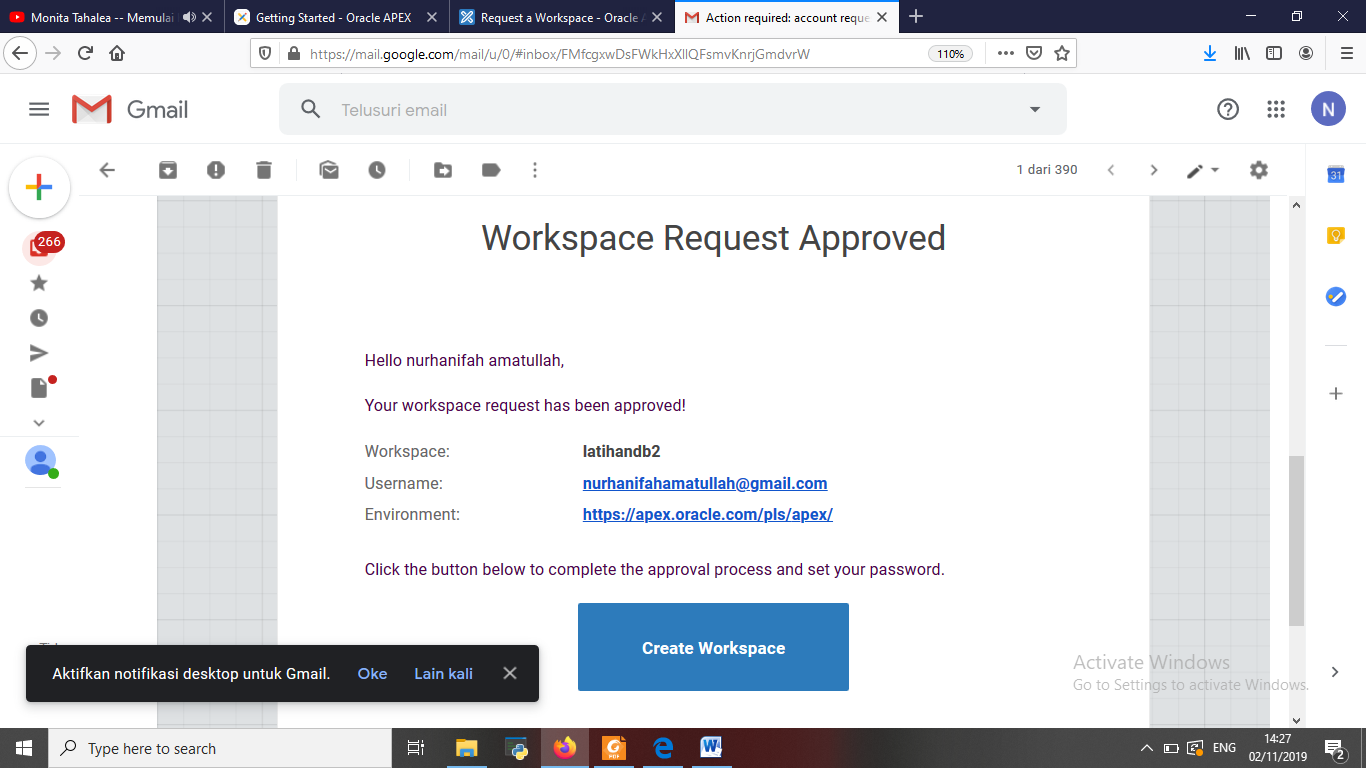
\includegraphics[scale = 0.3]{gambar/6.png}

\item Masuk ke menu SQL Workshop dan Pilih Object Browser. Kemudian Delete Column ID karena tidak digunakan dan akan digantikan dengan primmary key yang baru. Lakukan langkah ini untuk semua table\\
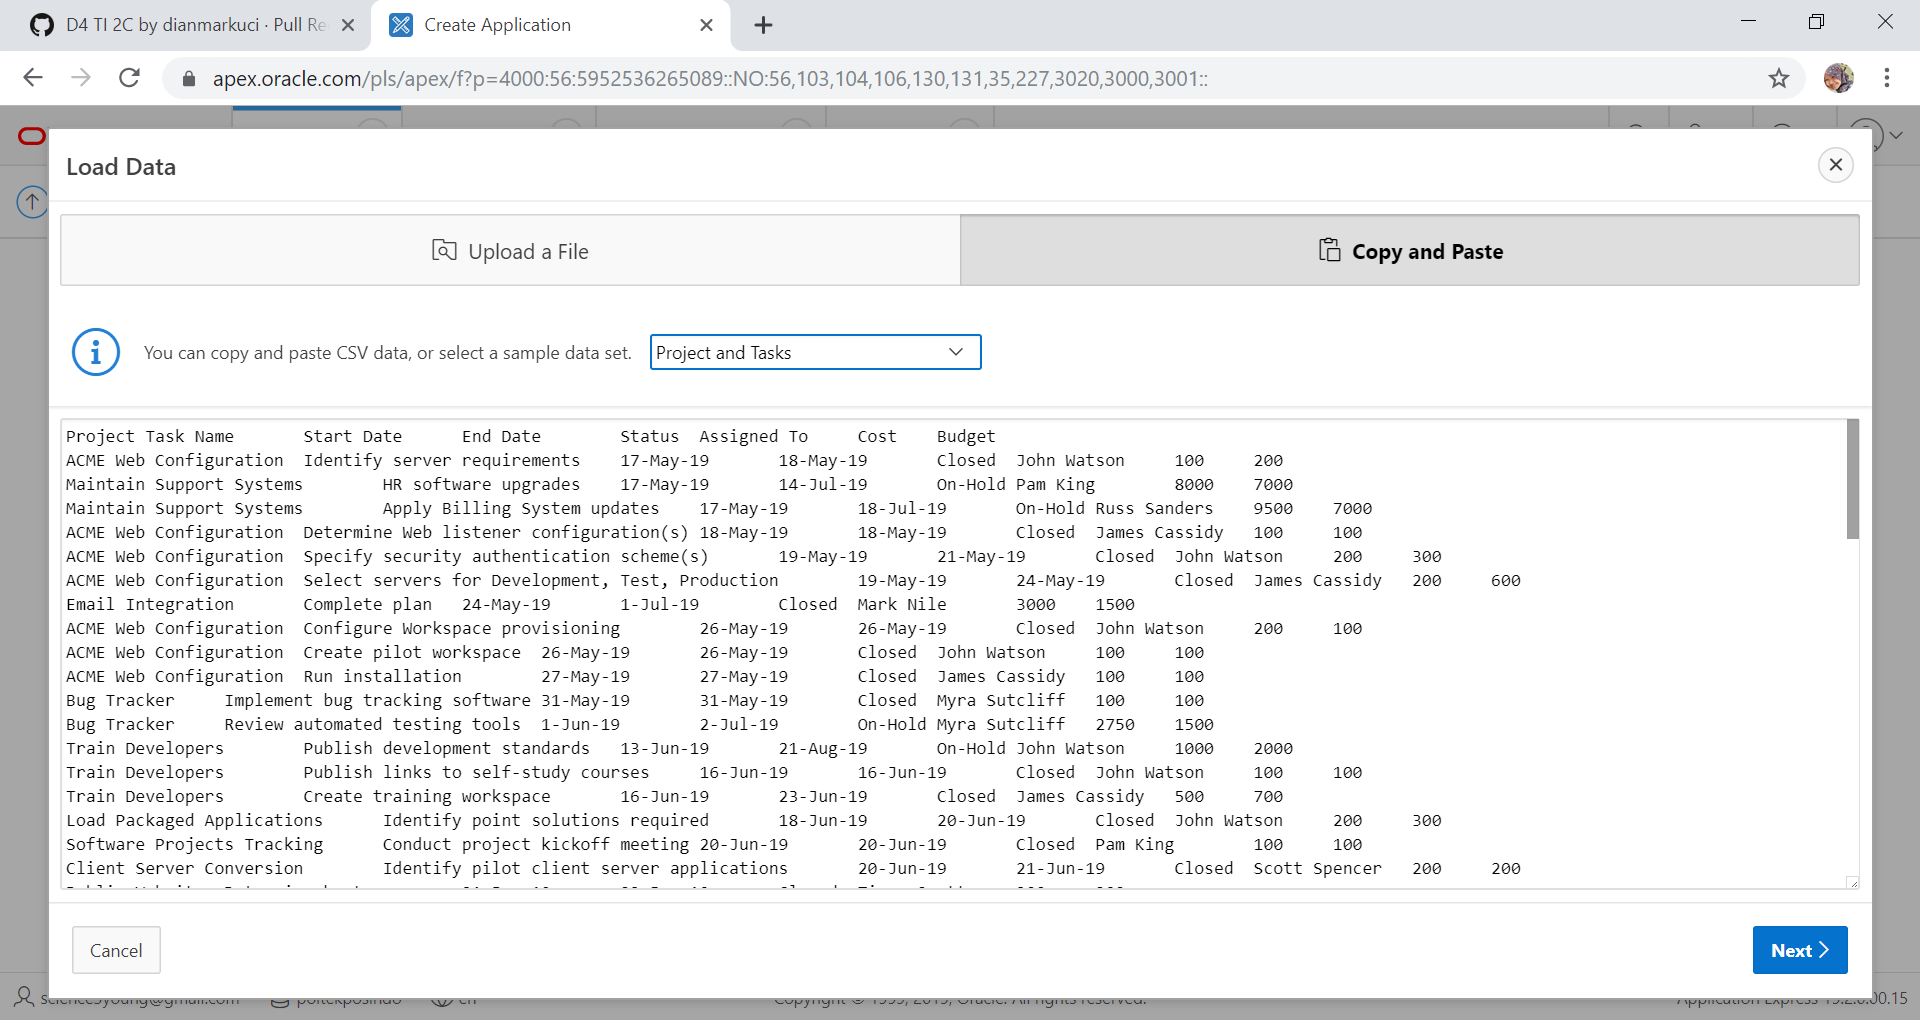
\includegraphics[scale = 0.3]{gambar/7.png}

\item Setelah semua ID dihapuskan, kemudian buka SQL Worksop, Klik SQL Command. kemudian inputkan perintah SQL untuk membuat primary key dan foreign key yang baru.\\
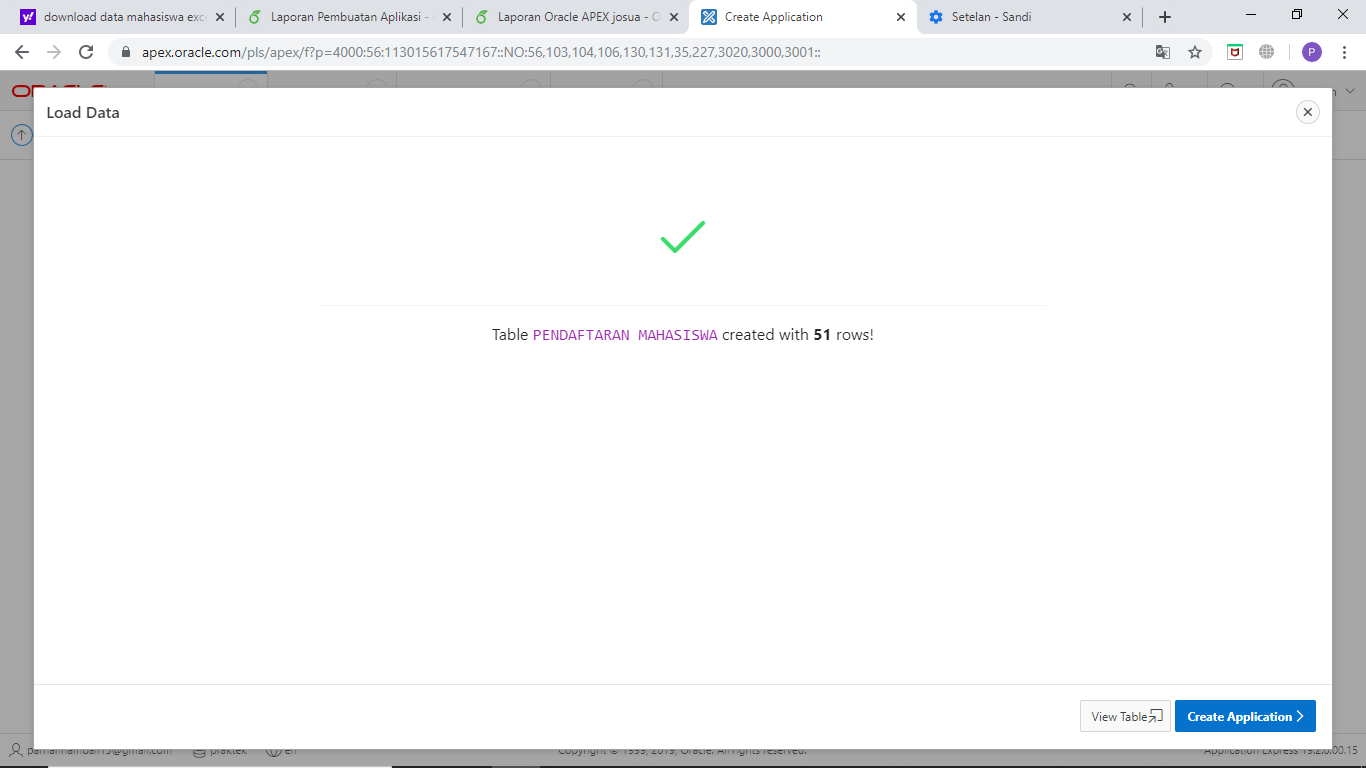
\includegraphics[scale = 0.3]{gambar/8.png}

Perintah SQL yang digunakan:\\
\begin{lstlisting}
ALTER TABLE ANGKATAN
ADD PRIMARY KEY (KODE_ANGKATAN);

ALTER TABLE MAHASISWA
ADD FOREIGN KEY (ANGKATAN) REFERENCES ANGKATAN (KODE_ANGKATAN);

ALTER TABLE PRODI
ADD PRIMARY KEY (KODE_PRODI);

ALTER TABLE MAHASISWA
ADD FOREIGN KEY (PRODI) REFERENCES PRODI (KODE_PRODI);

ALTER TABLE KELAS
ADD PRIMARY KEY (KODE_KELAS);

ALTER TABLE MAHASISWA
ADD FOREIGN KEY (KELAS) REFERENCES KELAS (KODE_KELAS);

ALTER TABLE JENJANG
ADD PRIMARY KEY (KODE_JENJANG);

ALTER TABLE MAHASISWA
ADD FOREIGN KEY (JENJANG) REFERENCES JENJANG (KODE_JENJANG);
\end{lstlisting}

\item Setelah input perintah SQL, kemudian kembali ke halaman awal. dan klik create application untuk membuat aplikasi. Masukan nama aplikasi dan Klik add page\\
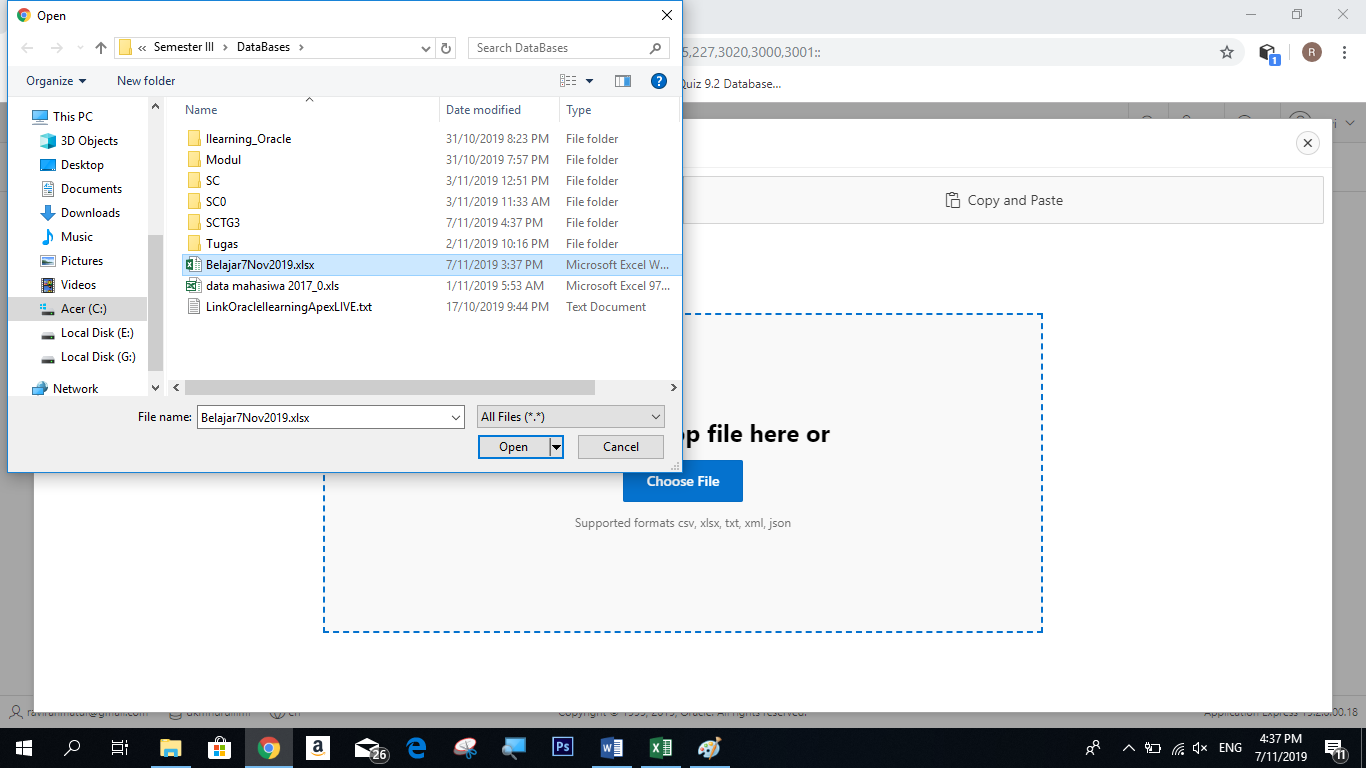
\includegraphics[scale = 0.3]{gambar/9.png}

\item Masukan page name dan table. Kemudian klik add page.\\
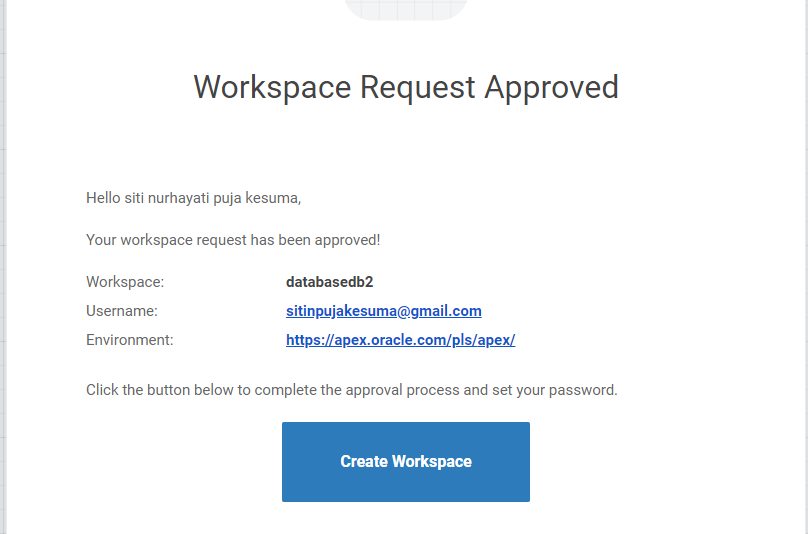
\includegraphics[scale = 0.3]{gambar/10.png}

\item Setelah semua ditambahkan, pergi ke halaman awal dan klik run application\\
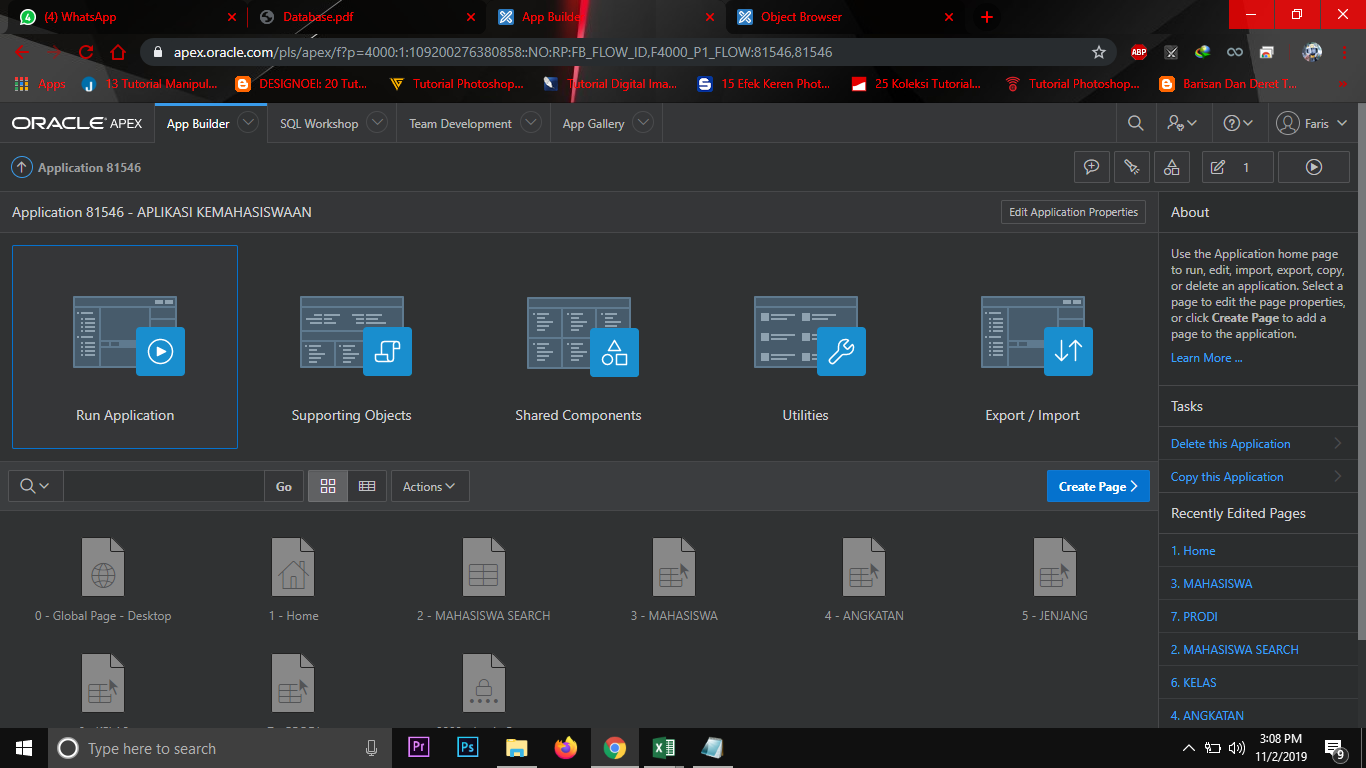
\includegraphics[scale = 0.3]{gambar/11.png}

\item Aplikasi Kemahasiswaan dapat di run\\
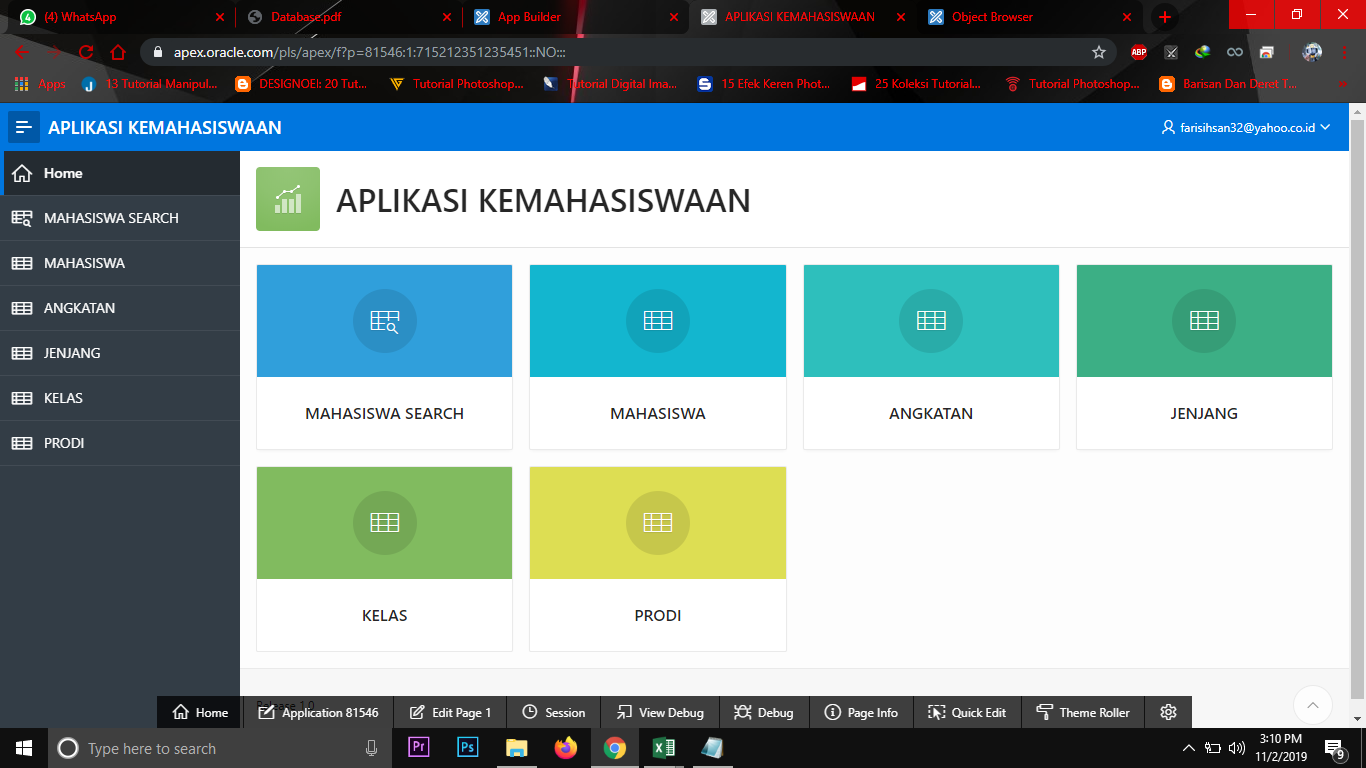
\includegraphics[scale = 0.3]{gambar/12.png}
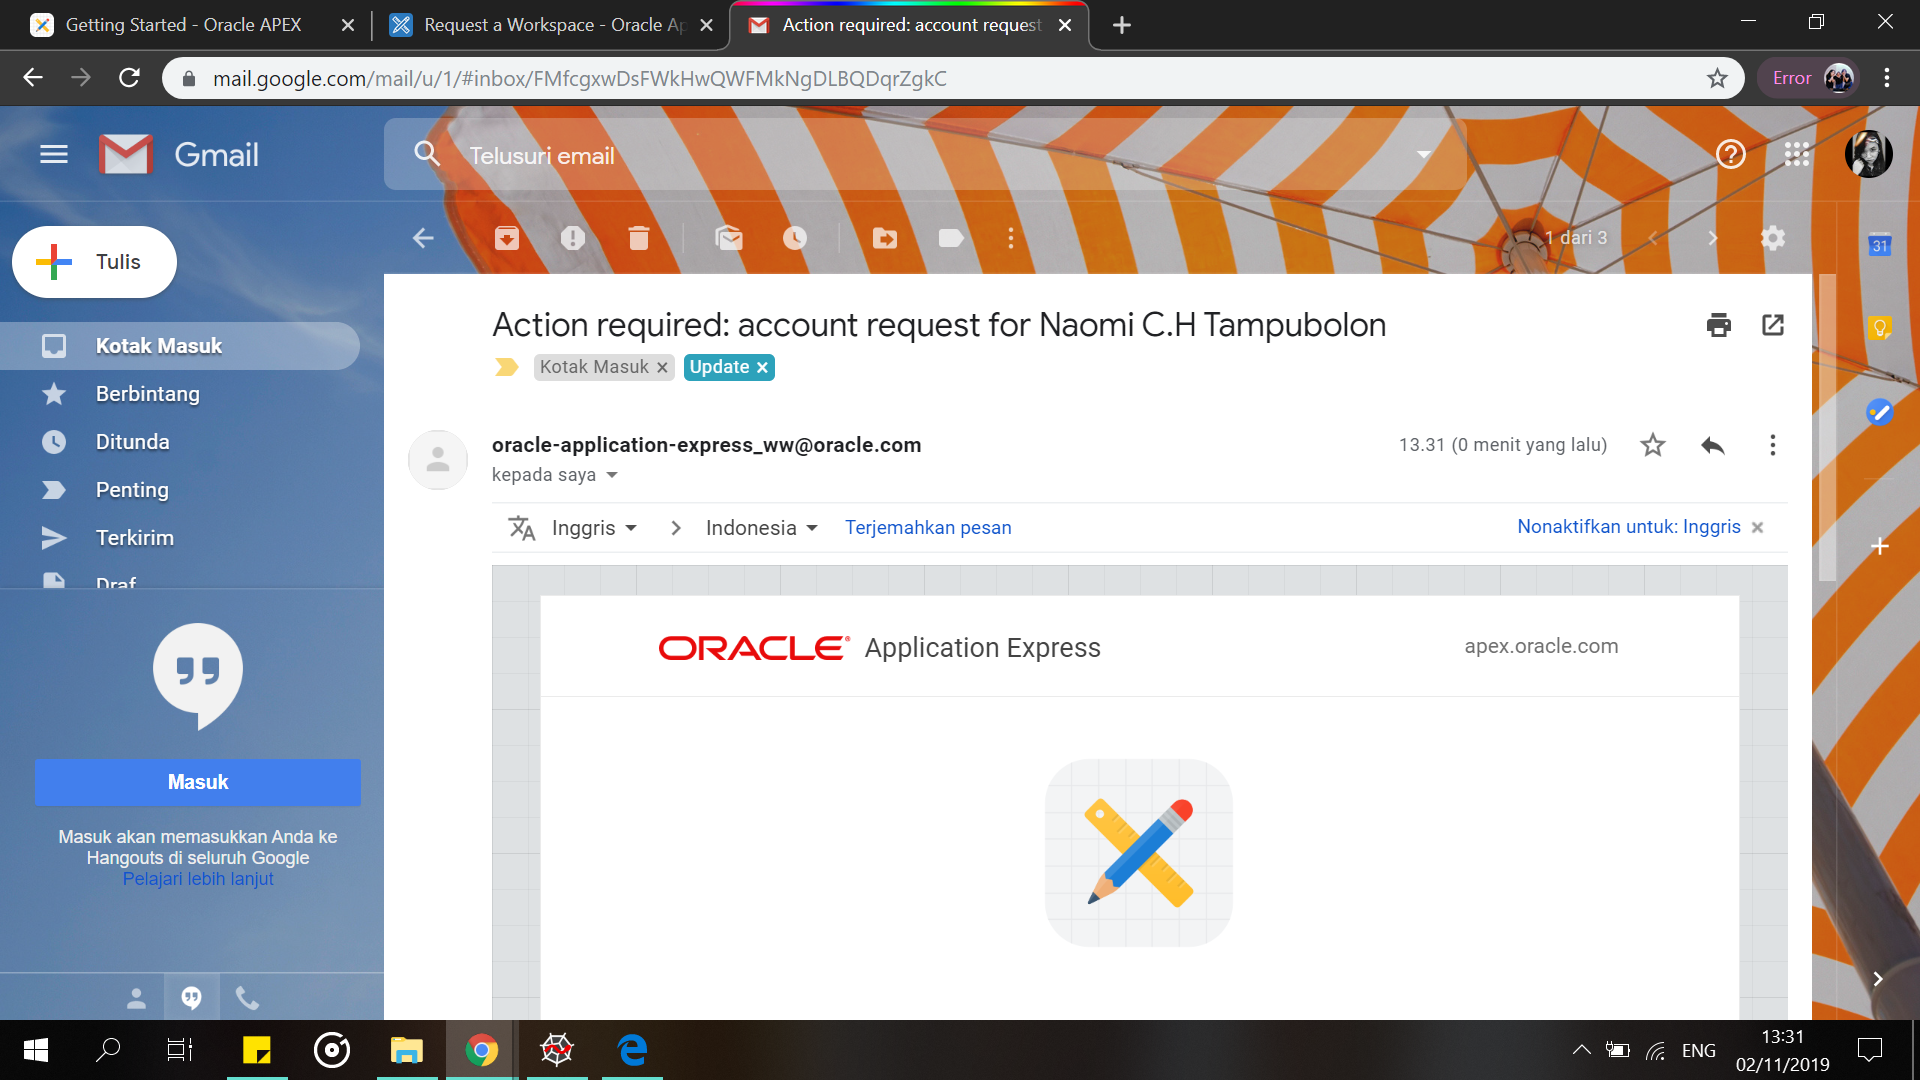
\includegraphics[scale = 0.3]{gambar/13.png}

\item \href {https://apex.oracle.com/pls/apex/f?p=81546:1:715212351235451::NO:::}{Link Aplikasi Mahasiswa}

\end{enumerate}



\end{document}

